\documentclass[10pt,twocolumn,letterpaper]{article}

\usepackage{cvpr}
\usepackage{times}
\usepackage{epsfig}
\usepackage{graphicx}
\usepackage{amsmath}
\usepackage{amssymb}

% Include other packages here, before hyperref.

% If you comment hyperref and then uncomment it, you should delete
% egpaper.aux before re-running latex.  (Or just hit 'q' on the first latex
% run, let it finish, and you should be clear).
\usepackage[breaklinks=true,bookmarks=false]{hyperref}

\cvprfinalcopy % *** Uncomment this line for the final submission

\def\cvprPaperID{****} % *** Enter the CVPR Paper ID here
\def\httilde{\mbox{\tt\raisebox{-.5ex}{\symbol{126}}}}

% Pages are numbered in submission mode, and unnumbered in camera-ready
%\ifcvprfinal\pagestyle{empty}\fi
\setcounter{page}{1}
\begin{document}

%%%%%%%%% TITLE
\title{Self-Driving Car Steering Angle Prediction Based on Image Recognition (Milestone)}

\author{Shuyang Du\\
{\tt\small shuyangd@stanford.edu}
% For a paper whose authors are all at the same institution,
% omit the following lines up until the closing ``}''.
% Additional authors and addresses can be added with ``\and'',
% just like the second author.
% To save space, use either the email address or home page, not both
\and
Haoli Guo\\
{\tt\small haoliguo@stanford.edu}
\and
Andrew Simpson\\
{\tt\small asimpso8@stanford.edu}
}

\maketitle
%\thispagestyle{empty}

%%%%%%%%% ABSTRACT
\begin{abstract}
   Self-driving vehicles have expanded drastically over the last few year. Udacity has release a dataset containing, among other data, a set of images with the steering angle captured during driving. The Udacity challenge aimed to predict steering angle based on only the provided images. We explore different models to perform high quality prediction of steering angles based only images using different deep learning techniques.
\end{abstract}

%%%%%%%%% BODY TEXT
\section{Introduction}
Self-driving vehicles are going to be of enormous economic impact over the coming decade. Creating models that meet or exceed the ability of a human driver could save thousands of lives a year. 

Udacity has an ongoing challenge to create an open source self-driving car. In their second challenge Udacity released a dataset of images taken while driving along with the corresponding steering angle and ancillary sensor data for a training set (left, right, and center cameras with interpolated angles based on camera angle). The goal of the challenge was to find a model that, given a image taken while driving, will minimize the RMSE (root mean square error) between what the model predicts and the actual steering angle produced by a human driver. From this challenge, several top models emerged. The top three teams had an RMSE of approximately 0.055 (a guess of the mean angle, 0, would predict 0.2067). We will explore a variety of techniques including 3D convolutional neural networks, recurrent neural networks using LSTM, ResNets, etc. to output a predicted steering angle in numerical values. 

The motivation of the project is to eliminate the need for hand-coding rules and instead create a system that learns how to drive by observing. Predicting steering angle is one important part of the end-to-end approach to self-driving car and would allow us to explore the full power of neural networks. For example, using only steering angle as the training signal, deep neural networks can automatically extract features to help position the road to make the prediction.



%-------------------------------------------------------------------------
\section{Related Work}

NVIDIA released a paper last year "End to End Learning for Self-Driving Cars" \cite{bojarski2016end}. In this paper the authors used a relatively basic CNN architecture. The layout of the architecture can be seen in Figure \ref{nvidiaimage}. Augmentation of the data collected was found to be important. The authors used artificial shifts and rotations of the training set. Left and right cameras with interpolated steering angles were also incorporated.
\begin{figure}[!htb]
	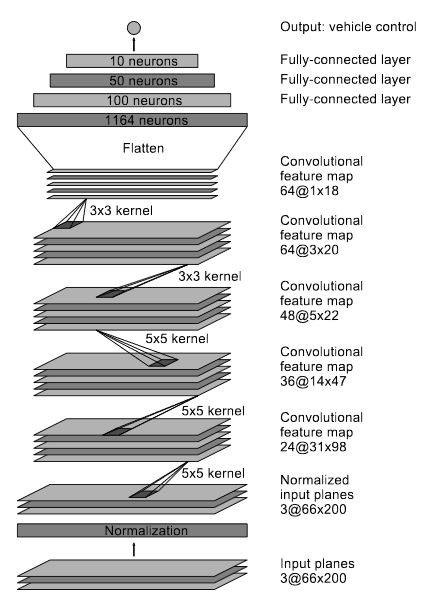
\includegraphics[width=6cm]{nvidiacnn}
	\centering
	\caption{CNN architecture used in \cite{bojarski2016end}. The network contains approximately 27 million connections and 250 thousand parameters.}
	\label{nvidiaimage}
\end{figure}


"Learning Spatiotemporal Features with 3D Convolutional Networks" introduces how to construct 3D Convolutional Networks to capture spatiotemporal features in a sequence of images or videos \cite{Tran_2015_ICCV}. "Beyond Short Snippets: Deep Networks for Video Classification" describes two ways including using LSTM to deal with videos \cite{yue2015beyond}.

"Deep Residual Learning for Image Recognition" \cite{he2016deep} and "Densely Connected Convolutional Networks" \cite{huang2016densely} describe the techniques to construct residual connections between different layers and make it easier to train deep neural networks. 


\section{Methods}

We investigated the top three existing models from the Udacity challenge to study how they work. The first examined model from the challenge is based on Team Komanda's model. The model performs a mapping from sequences of images (or one single video) to sequences of steering angles. Although the target is only the steering angle, this model predicts not only the steering angle, but also the vehicle speed and the torque applied to the steering wheel, which would be used to predict future steering angle. 

The model is consisted by a 3D convolutional stack and a RNN (LSTM) layer after it. The 3D convolutional stack contains four 3D convolutional layers followed by several fully connected layers, converting to a vector with 128 activations in the end. Each 3D convolutional layer will also produce an auxiliary output to be added to the final fully connected layer (residual connect). The output from this 3D convolutional stack will have shape (batch\_size, seq\_len, 128).

How 3D convolutional layer works is similar to 2D conv, the only difference is that in addition to height and width, now we have the third dimension depth. Instead of having a 2D filter (if we ignore the channel dimension for a while) moving within the image along height and width, now we have a 3D filter moving along with height, width and depth. If the input has shape ($D_{1}$, $H_{1}$,  $W_{1}$, $C$), then the output would have shape ($D_{2}$, $H_{2}$, $W_{2}$, $F$) where $F$ is the number of filters. ($D_{2}$, $H_{2}$, $W_{2}$ could be calculated given stride and padding in its dimension.

Combining the output from 3D convolutional layer stack and previous predicted steering angle, torque and speed, we have the input to RNN layer. This input is a tuple of two tensors with shape (batch\_size, seq\_len, 128) and (batch\_size, seq\_len, 3). Based on this input, RNN will make predictions for steering angle, torque and speed. 

The final loss is consisted of major loss from steering angle prediction and auxiliary loss from torque and speed. 
$loss=L2(steering angle)+auxiliary weight*(L2(steering angle)+L2(torque)+L2(speed))$

The L2 loss here is the loss across both batch\_size and seq\_len as we have the true label for each point in the sequence.

During training, we use both ground truth and previous predicted angle, torque and speed as our input to RNN. During testing, we only use previous prediction as the input to RNN.
\begin{figure}[!htb]
	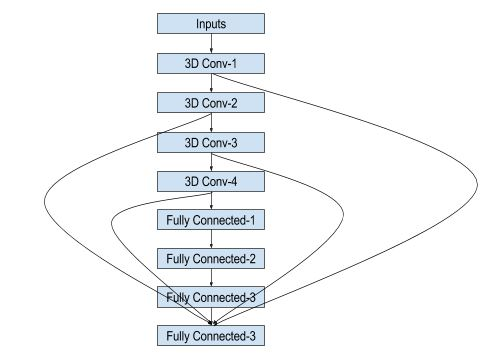
\includegraphics[width=6cm]{Komanda.JPG}
	\centering
	\caption{Architecture used for team Komanda.}
	\label{komanda}
\end{figure}

The next model we examined from the challenge was from Team Rambo. To preprocess the data, the images were converted to grayscale and lag 1 differences between frames were computed. Two consecutive differenced images were used as the input of the model. For example, at time $t, [x_{t} - x_{t-1}, x_{t-1} - x_{t-2}]$ is used as input where x corresponds to the grayscale image. Since two consecutive differenced images were used, the number of channels is 2, but this is a hyperparameter for tuning. 

In the training process, the model consists of 3 streams that are assembled at the final layer. Figure \ref{rambo} shows the architecture of the model. 
\begin{figure}[!htb]
	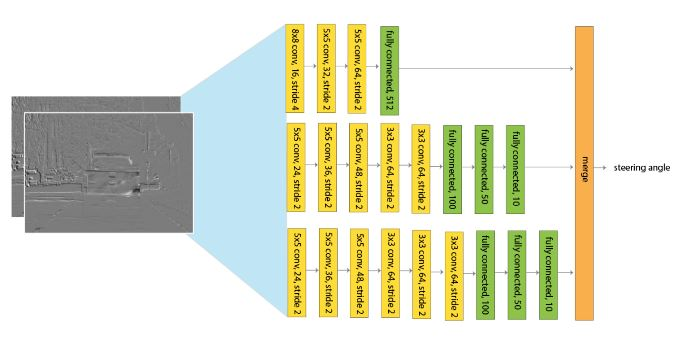
\includegraphics[width=6cm]{rambo.JPG}
	\centering
	\caption{Architecture used for team Rambo.}
	\label{rambo}
\end{figure}
Each stream of the model consists of a sequence of convolutional layers, interspersed with activation functions such as ReLU, Leaky ReLU or Parametric ReLU (PReLU). Adam optimization and L2 loss were adopted as the optimization method and loss equation.

A third model from team Chauffeur was examined. This team placed third with an RMSE of 0.0572. This model had a core structure that was similar to that of team Komanda with the exception of not using 3D convolutional networks. This team used a large pretrained CNN model. This model was then modified to have an output of approximately 3000 features that was then passed into a relatively simple LSTM (long short-term memory \cite{hochreiter1997long}) network with the best model having a window of 50 images or 2.5 seconds of video.



\subsection{Potential Methods}

A potential method is taking the last $n$ frames from the training set allow use of networks using 3D convolutions \cite{Tran_2015_ICCV}. Creating an architecture like ResNet with these 3D layers may capture important image information between layers and let the gradient pass back deeper into the network. Additionally passing the processed data from this network into an RNN (using LSTM) could allow for knowledge of the previous states to be used to predict the next state of the steering angle. Additional methods that different teams used that could be used with this approach is to take the difference between frames instead of the raw image data. Transfer learning of a large network would also likely be helpful for model development. Ideally, if a high quality simulator can be found, this trained network can modified to be used for deep reinforcement learning. After training in the simulator the model can then be evaluated on the validation and test sets.

\subsection{Data Preprocessing}
During experimentation, copying the general structure from \cite{bojarski2016end} with the dataset from Udacity produced poor results. Initially, training data was passed unprocessed into the model. Without any preprocessing, the RMSE on the training set was very low; however, the error on the validation set was worse than passing all zeros in as the output (0.2130 on the validation set). We are currently examining ways to best augment the training set to improve performance on the validation set. One common idea in the different teams was to flip the training on the $y$ axis to account for any turn asymmetry. Adding random shadows, hue changes, rotations, and shifts in the images are being examined along with incorporation images from the left and right cameras. However, using the left and right cameras when using RNNs may not make sense as the angle is interpolated as what the car should do if that image were the front facing camera. Frames that have the steering angle at approximately 0 can be preferentially excluding in favor of frames with larger steering angles.


\section{Dataset and Features}
The dataset we used is provided by Udacity, which is generated by NVIDIA’s DAVE-2 System \cite{bojarski2016end}. Specifically, three cameras are mounted behind the windshield of the data-acquisition car. Time-stamped video from the cameras is captured simultaneously with the steering angle applied by the human driver. This steering command is obtained by tapping into the vehicle’s Controller Area Network (CAN) bus. In order to make the system independent of the car geometry, they represent the steering command as 1/r where r is the turning radius in meters. They use 1/r instead of r to prevent a singularity when driving straight (the turning radius for driving straight is infinity). 1/r smoothly transitions through zero from left turns (negative values) to right turns (positive values). Training data contains single images sampled from the video, paired with the corresponding steering command (1/r).

In addition to the images got from the center camera, images for two specific off-center shifts can be obtained from the left and the right camera. Additional shifts between the cameras and all rotations are simulated by viewpoint transformation of the image from the nearest camera. This could be regarded as a way we used to augment the data.

Raw images are of size 640 x 480 and have three channels RGB. For one of our models, we resized the images to 256 x 192, converted from RGB color format to grayscale, computed lag 1 differences between frames and used 2 consecutive differenced images. For example, at time t we used $[x_{t} - x_{t-1}, x_{t-1} - x_{t-2}]$ as input where x corresponds to the grayscale image.

Training data set contains 101397 frames and corresponding labels including steering angle, torque and speed. We further split this data set into training and validation in a 80/20 fashion. And there is also a test set which contains 5615 frames. 

\section{Experiments, Results, and Discussion}
As a baseline, the work from \cite{bojarski2016end} is being reproduced on the dataset from Udacity. A model, using Keras, was constructed that followed the layout from \cite{bojarski2016end}. Currently the results have only produced a result of 0.19 on the validation set. This result is better than guessing all zeros, but is not a competitive score. Further data augmentation is being examined to improve the RMSE on the validation set.

Additionally, as preliminary results, we succeed to make our model overfit on a small training data set. With training on larger data set on single GPU Google Cloud Instance for 10 hours, we achieved 0.2 RMSE for steering angle prediction on validation set. However, the error on validation set is strangely nonmonotonic. As we trained model, even without overfitting, the error on validation set changed non monotonically.

Team Chauffeur's code was examined and reproduced. In testing this code it was found to have a high RMSE at first, but eventually produced quality results (RMSE 0.0672). The core idea of this model can likely be extended to other methods such as 3D convolution with temporal data. This may or may not aid the later LSTM network, which would, by its own architecture, contain temporal information.

In examining these models we think it would be possible to combine different aspects in order to obtain similar or superior results. 


\section{Conclusion and Future Work}
Finding better ways to augment the training dataset allows for an effectively larger training set size, which will help better generalization on the validation and testing sets. Exploring new models using the latest techniques may elucidate superior results.


{\small
\bibliographystyle{ieee}
\bibliography{egbib}
}

\end{document}
